\documentclass{article}
\usepackage{xeCJK} 
\usepackage{amsmath}
\usepackage{amsfonts}
\usepackage{amssymb}
\usepackage{graphicx} 
\usepackage{tikz}

\setCJKmainfont{SimSun}[AutoFakeBold,AutoFakeSlant]

\usetikzlibrary{shapes.geometric, arrows}

\tikzstyle{startstop} = [rectangle, rounded corners, minimum width=3cm, minimum height=1cm, text centered, draw=black, fill=red!30]
\tikzstyle{process} = [rectangle, minimum width=3cm, minimum height=1cm, text centered, draw=black, fill=blue!20]
\tikzstyle{decision} = [diamond, minimum width=3.5cm, minimum height=1cm, text centered, draw=black, fill=green!20]
\tikzstyle{arrow} = [thick,->,>=stealth]

\begin{document}
\title{PRML第四次作业}
\author{许书闻 2023K8009926005}
\maketitle

\section*{第1题}
(1)
(i)贝叶斯最小错误率决策规则:
\[\min_{decision}P(error)=\int P(error|\boldsymbol{x})p(\boldsymbol{x})dx\]
例如当$c=2$时的二分类问题中:

\[P(error|\boldsymbol{x})=
\begin{cases}
    1-P(\omega_1|\boldsymbol{x})=P(\omega_2|\boldsymbol{x}),&x\in \omega_1\\
    1-P(\omega_2|\boldsymbol{x})=P(\omega_1|\boldsymbol{x}),&x\in \omega_2\\
\end{cases}
\]
决策规则:
\[x \in
\begin{cases}
    \omega_1,~~if P(\omega_1|\boldsymbol{x})\geq P(\omega_2|\boldsymbol{x})\\
    \omega_2,~~if P(\omega_2|\boldsymbol{x})> P(\omega_1|\boldsymbol{x})\\
\end{cases}
\]
由Bayes公式,\[P(\omega_i|\boldsymbol{x})=\frac{P(\boldsymbol{x}|\omega_i)P(\omega_i)}{P(\boldsymbol{x})}\]可知\(P(\omega_i|\boldsymbol{x})\)正比于\(P(\omega_i|\boldsymbol{x})P(\omega_i)\),所以决策规则也可以写作:
\[x \in
\begin{cases}
    \omega_1,~~if P(\omega_1|\boldsymbol{x})P(\omega_1)\geq P(\omega_2|\boldsymbol{x})P(\omega_2)\\
    \omega_2,~~if P(\omega_2|\boldsymbol{x})P(\omega_2)> P(\omega_1|\boldsymbol{x})P(\omega_1)\\
\end{cases}
\]
等价地,若\(l(\boldsymbol{x})=\frac{p(\boldsymbol{x}|\omega_1)}{p(\boldsymbol{x}|\omega_2)}
\begin{cases}
    <t=\frac{p(\omega_2)}{p(\omega_1)},\\
    >t=\frac{p(\omega_2)}{p(\omega_1)},\\
\end{cases}\)
则\(\boldsymbol{x}\in
\begin{cases}
\omega_1\\
\omega_2\\
\end{cases} 
\)

其中$l(\boldsymbol{x})$称为似然比(liklihood ratio), $P(\boldsymbol{x}|\omega_i)P(\omega_i)$称为似然度(liklihood).

当$c\geq3$时,多类最小错误率决策:\\
平均错误率:\[P(e|\alpha_j)=\sum_{i=1,i\neq j}^{c}P(\omega_i|\boldsymbol{x})=1-P(\omega_j|\boldsymbol{x})\]
如果设$\alpha_j$表示决策为$\omega_j$\\
\[P(e|\alpha_j)=\sum_{i=1,i\neq j}^{c}P(\omega_i|\boldsymbol{x})=1-P(\omega_j|\boldsymbol{x})\]
最小错误率决策也为最大后验概率决策(MAP)\[P(\omega_i|\boldsymbol{x})=\max_{j=1,2,...,c}P(\omega_j|\boldsymbol{x})\Rightarrow x\in \omega_i\]
等价地,\[P(\boldsymbol{x}|\omega_i)P(\omega_i)=\max_{j=1,2,...,c}P(\boldsymbol{x}|\omega_j)P(\omega_j)\Rightarrow x\in \omega_i\]

(ii)最小风险决策:
输入特征向量$\boldsymbol{x}=[x_1,x_2,...,x_n]^{T}$,类别集为$\Omega=\{\omega_1,\omega_2,...,\omega_c\}$,决策空间为$A=\{\alpha_1,\alpha_2,...,\alpha_k\}$(k可能等于c,或有拒识的情况下大于c),决策代价为$\lambda(\alpha_i,\omega_j)=\lambda_{ij}$.

决策方法为$\alpha_i$的条件风险:
\[R(\alpha_i|\boldsymbol{x})=\sum_{j=1}^{c}\lambda(\alpha_i,\omega_j)P(\omega_j|\boldsymbol{x}),i=1,...,k\]最小风险Bayes决策:
\[if~R(\alpha_i|\boldsymbol{x})=\min_{j=1,...,k}R(\alpha_j|\boldsymbol{x}),~~~~then~\alpha\in\alpha_i\]
(2)考虑拒识的情况,拒识为第$c+1$类,由题意,风险函数可定义为:
\[\lambda(\alpha_i,\omega_j)=
\begin{cases}
    0,~~i=j,i\leq c\\
    \lambda_s,~~i\neq j,i\leq c\\
    \lambda_r,~~i=c+1\\
\end{cases}    
\]
条件风险为:
\[R(\alpha_j|\boldsymbol{x})=\sum_{j=1}^{c}\lambda(\alpha_i,\omega_j)P(\omega_j|\boldsymbol{x})=
\begin{cases}
    \lambda_s-\lambda_sP(\omega_i|\boldsymbol{x}),~~i\leq c\\
    \lambda_r,~~i=c+1\\
\end{cases}    
\]
对应的决策规则为
\[
\begin{cases}
    x\in \omega_i,~~~P(\omega_i|\boldsymbol{x})=\max_{j=1,...,c} P(\omega_j|\boldsymbol{x})>1-\frac{\lambda_r}{\lambda_s}\\
    Reject,~~~otherwise\\
\end{cases} 
\]
(3)拒识的意义:

1. 提高分类器的可靠性: 拒识可以避免在分类器不确定时做出错误的决策,特别是在模型对某些输入样本没有足够信心的情况下。

2. 减少错误分类: 当输入样本远离训练数据的分布时,拒识可以防止将这些样本错误分类为某个类别,从而减少误分类的风险。

2. 更高的精确度: 拒识策略有助于提升分类的精度,因为只有在模型非常有信心的情况下才会做出分类决策。

拒识的应用场景有:

医疗诊断: 如果分类器对某个病例的诊断结果不确定,可能会选择拒绝诊断,而让医生进一步检查,而不是做出错误的诊断。

信用卡欺诈检测: 在一些情况下,分类器可能会拒绝判断某个交易是否欺诈,以避免错误地标记合法交易为欺诈。

垃圾邮件检测: 如果模型无法明确判断一封邮件是否为垃圾邮件,拒识策略可以避免错误标记。

\section*{第2题}

(1)类条件概率密度函数的数学形式:
\[p(\boldsymbol{x}|\omega_i)=\frac{1}{(2\pi)^{d/2}|\boldsymbol{\Sigma_i}|^{1/2}}\exp\{-\frac{1}{2}(\boldsymbol{x}-\boldsymbol{\mu_i})^T\Sigma_i^{-1}(\boldsymbol{x}-\boldsymbol{\mu_i})\}\]
其中$\mu=E\{\boldsymbol{x}\}$,$\Sigma_i=E\{(\boldsymbol{x}-\boldsymbol{\mu_i})(\boldsymbol{x}-\boldsymbol{\mu_i})^T\}$

(2)
Bayes决策准则即选择最大后验概率:
\[\alpha_j=argmax_{i} P(\omega_i|\boldsymbol{x})\propto p(\boldsymbol{x}|\omega_i)p(\omega_i)\]
由于先验相等,只需最大化$p(\boldsymbol{x|\omega_i})$,定义对数判别函数:
\[g_i(\boldsymbol{x})=2\ln p(\boldsymbol{x}|\omega_i)p(\omega_i)=-(\boldsymbol{x}-\boldsymbol{\mu_i})^T\Sigma_i^{-1}(\boldsymbol{x}-\boldsymbol{\mu_i})-d\cdot \ln2\pi-\ln|\Sigma_i|+2\ln p(\omega_i)\]下面讨论各类协方差矩阵是否相等

(i)类协方差矩阵相等$(\Sigma_i=\Sigma)$,忽略与i无关项:
\[g_i(\boldsymbol{x})\equiv 2\boldsymbol{\mu}_i^T\Sigma^{-1}\boldsymbol{x}-\boldsymbol{\mu_i}^T\Sigma^{-1}\boldsymbol{\mu}_i+2\ln p(\omega_i)\]

(ii)类协方差矩阵不等$(\Sigma_i\neq\Sigma)$,忽略与i无关项:
\[g_i(\boldsymbol{x})=-(\boldsymbol{x}-\boldsymbol{\mu_i})^T\Sigma_i^{-1}(\boldsymbol{x}-\boldsymbol{\mu_i})-\ln|\Sigma_i|+2\ln p(\omega_i)=\boldsymbol{x}^T\boldsymbol{W}_i\boldsymbol{x}+\boldsymbol{w}_i^T\boldsymbol{x}+\omega_0\]

其中$\boldsymbol{W_i}=-\Sigma_i^{-1}$, $\boldsymbol{w}_i=2\Sigma_i^{-1}\boldsymbol{\mu_i}$, $\omega_{i0}=-\boldsymbol{\mu_i}^T\Sigma_i^{-1}\boldsymbol{\mu_i}-\ln|\boldsymbol{\Sigma_i}|+2\ln p(\omega_i)$

(3)两类等协方差矩阵情况下,各类样本分别集中于以该类均值$\mu_i$为中心的同样大小和形状的超椭球内,决策面是一个线性超平面,决策面的位置与类的均值有关,决策面法向量是$\boldsymbol{\Sigma^{-1}(\mu_1-\mu_2)}$

若两类的先验概率相等,决策面经过$\boldsymbol{\mu}_1$和$\boldsymbol{\mu_2}$连线的中点;

若两类的先验概率不相等,决策面会向着先验概率小的均值点偏移。

(4)当协方差矩阵 $\Sigma$ 为奇异矩阵时,可以采用正则化方法使其可逆。正则化后的协方差矩阵表示为:
\[
\Sigma_{\text{reg}} = \Sigma + \lambda I
\]
其中:
\begin{itemize}
  \item $\Sigma$ 是原始协方差矩阵;
  \item $\lambda > 0$ 是一个很小的正数(正则化参数);
  \item $I$ 是与 $\Sigma$ 同阶的单位矩阵。
\end{itemize}

此时,$\Sigma_{\text{reg}}$ 是正定矩阵,因而可以进行逆运算:
\[
\Sigma_{\text{reg}}^{-1} = (\Sigma + \lambda I)^{-1}
\]

\section*{第3题}
HMM的例子:天气预测和人们的穿衣情况

我们无法直接观察天气状态,但可以通过某人每天的穿衣情况来间接推测当地的天气。这个过程可建模为一个隐马尔可夫模型(HMM)。

\subsection*{1. HMM组成对应关系}

\begin{itemize}
  \item \textbf{隐状态(Hidden States)}:天气情况 \\[3pt]
    \[
    S = \{\text{晴天}, \text{多云}, \text{雨天} \}
    \]
    
  \item \textbf{观测变量(Observations)}:穿衣类型 \\[3pt]
    \[
    O = \{\text{短袖}, \text{长袖}, \text{外套}, \text{雨衣} \}
    \]
    
  \item \textbf{状态转移概率矩阵 $A$}:天气之间的转移概率 \\[3pt]
    \[
    A = 
    \begin{bmatrix}
    P(\text{晴} \rightarrow \text{晴}) & P(\text{晴} \rightarrow \text{多云}) & \cdots \\
    P(\text{多云} \rightarrow \text{晴}) & P(\text{多云} \rightarrow \text{多云}) & \cdots \\
    \vdots & \vdots & \ddots
    \end{bmatrix}
    \]
    
  \item \textbf{观测概率矩阵 $B$}:在某种天气下穿某类衣服的概率 \\[3pt]
    \[
    B = 
    \begin{bmatrix}
    P(\text{短袖}|\text{晴}) & P(\text{长袖}|\text{晴}) & \cdots \\
    P(\text{短袖}|\text{多云}) & P(\text{长袖}|\text{多云}) & \cdots \\
    \vdots & \vdots & \ddots
    \end{bmatrix}
    \]
    
  \item \textbf{初始状态概率向量 $\pi$}:第一天的天气分布 \\[3pt]
    \[
    \pi = \left[ P(\text{晴}), P(\text{多云}), P(\text{雨}) \right]
    \]
\end{itemize}

\subsection*{2. 示例观测序列}

假设某人连续五天朋友圈照片中的穿衣情况为:
\[
O = (\text{短袖}, \text{外套}, \text{雨衣}, \text{雨衣}, \text{长袖})
\]

我们希望通过此观测序列推测他那边每天的天气变化。

\subsection*{3. HMM的三类基本问题对应实际含义}

\begin{itemize}
  \item \textbf{观测序列评价(Likelihood Evaluation)}:\\
    给定模型 $\lambda = (A, B, \pi)$,计算观测序列出现的概率
    \[
    P(O|\lambda)
    \]
    对应问题:这套衣服组合是否符合某种天气变化的常见规律?是否异常?

  \item \textbf{状态序列解码(Decoding)}:\\
    给定观测序列,求最可能的隐状态序列 $Q = (q_1, q_2, \dots, q_T)$
    \[
    Q^* = \arg\max_Q P(Q|O, \lambda)
    \]
    对应问题:推断这五天每天的天气情况(例如使用 Viterbi 算法)。

  \item \textbf{参数学习(Learning)}:\\
    给定观测序列,估计最优模型参数 $(A, B, \pi)$
    \[
    \lambda^* = \arg\max_\lambda P(O|\lambda)
    \]
    对应问题:通过大量穿衣数据学习一个城市天气变化的规律。
\end{itemize}

\section*{第4题}
(1)概率密度估计方法
\subsection*{概率密度的参数估计}

(i)最大似然估计:
用一类的样本 $X = \{x_1, x_2, \ldots, x_N\}$ 估计一类概率密度函数的参数 $p(x|\theta)$。

样本集的似然度为
\[
L(\theta) = p(X|\theta) = p(x_1, x_2, \ldots, x_N|\theta) = \prod_{i=1}^{N} p(x_i|\theta)
\]
其中 $L(\theta)$ 表示样本集的似然度(likelihood),即 $p(x|\theta)$ 覆盖该样本集的程度。

最大似然估计步骤:
\begin{itemize}
    \item 找到参数 $\theta$ 使得 $L(\theta)$ 最大,记为 $\hat{\theta}$。$\hat{\theta} = d(x_1, x_2, \ldots, x_N)$ 是样本集的函数。
    \item $\hat{\theta}$ 即为最大似然估计,还可定义对数似然函数:
    \[
    H(\theta) = \ln L(\theta)
    \]
\end{itemize}

最大似然估计的求解:
\begin{itemize}
    \item 如果似然函数连续可微,则是下列函数的解:
    \[
    \frac{dL(\theta)}{d\theta} = 0 \quad \text{或} \quad \frac{dH(\theta)}{d\theta} = 0
    \]
    \item 更一般地,若 $\hat{\theta} = [\theta_1, \theta_2, \ldots, \theta_s]^T$,需使用以下偏导:
    \[
    \nabla_\theta = \left[ \frac{\partial}{\partial \theta_1}, \frac{\partial}{\partial \theta_2}, \ldots, \frac{\partial}{\partial \theta_s} \right]^T
    \]
    \[
    \nabla_\theta L(\theta) = 0 \quad \text{或} \quad \nabla_\theta H(\theta) = 0
    \]
    \item $\nabla_\theta L(\theta) = 0$ 是一个方程组,有时候可以解析求解;有时候不能,则需用梯度上升(gradient ascent)法进行迭代估计。
\end{itemize}
(ii)Bayes估计法:

\begin{itemize}
  \item 把参数估计看成贝叶斯决策问题;
  \item 估计参数看成具有先验分布 $p(\theta)$ 的随机变量;
  \item 其取值依据样本有关 $X = \{x_1, x_2, \dots, x_N\}$;
  \item 在先验分布与样本观测值条件下,损失函数为 $\lambda(\hat{\theta}, \theta)$。
\end{itemize}

用贝叶斯估计时的总期望风险为:
\[
R(\hat{\theta}) = \int_{\theta} \left[ \int_{x} \lambda(\hat{\theta}(x), \theta) p(x|\theta) dx \right] p(\theta) d\theta
\]
定义在样本 $X$ 下的条件风险为:
\[
R(\hat{\theta}|x) = \int_{\theta} \lambda(\hat{\theta}(x), \theta) p(\theta|x) d\theta
\]
总风险:
\[
R(\hat{\theta}) = \int_{x} R(\hat{\theta}|x) p(x) dx
\]
对经验风险最小,得到最优参数 $\hat{\theta}^*$。

常用平方损失函数:
\[
\lambda(\hat{\theta}, \theta) = (\hat{\theta} - \theta)^2
\]
可以证明:若采用平方误差损失函数,则贝叶斯估计量为条件期望
\[
\hat{\theta}^* = E(\theta|x) = \int_{\theta} \theta p(\theta|x) d\theta
\]
其中
\[
p(\theta|x) = \frac{p(x|\theta)p(\theta)}{p(x)} \quad , \quad p(x) = \int p(x|\theta)p(\theta) d\theta
\]
平方误差下贝叶斯估计的步骤:

\begin{itemize}
  \item 确定先验分布密度 $p(\theta)$;
  \item 求出样本集的联合分布:
  \[
  p(X|\theta) = \prod_{i=1}^{N} p(x_i|\theta)
  \]
  \item 利用贝叶斯公式求出参数后验概率(后验分布):
  \[
  p(\theta|X) = \frac{p(X|\theta)p(\theta)}{p(X)} \quad , \quad p(X) = \int p(X|\theta)p(\theta) d\theta
  \]
  \item 求贝叶斯估计量:
  \[
  \hat{\theta}^* = E(\theta|X)
  \]
  \item 贝叶斯估计得到的概率密度函数:
  \[
  p(x|X) = \int p(x|\theta)p(\theta|X) d\theta
  \]
\end{itemize}

递推贝叶斯估计(贝叶斯学习)

考虑样本数量逐渐增加的情况:
\[
X^N = \{x_1, x_2, \dots, x_{N-1}, x_N\} = \{X^{N-1}, x_N\}
\]

\[
p(\theta|X^N) = \frac{p(x_N|\theta)p(\theta|X^{N-1})}{p(x_N|X^{N-1})}
\]
其中
\[
p(x_N|X^{N-1}) = \int p(x_N|\theta)p(\theta|X^{N-1}) d\theta
\]
当 $N=1$ 时:
\[
p(\theta|x_1) = \frac{p(x_1|\theta)p(\theta)}{p(x_1)} \quad , \quad p(x_1) = \int p(x_1|\theta)p(\theta) d\theta
\]
可得如下递推公式:
\[
p(\theta|X^N) = \frac{p(x_N|\theta)p(\theta|X^{N-1})}{\int p(x_N|\theta)p(\theta|X^{N-1}) d\theta}
\]
样本充分多时:
\[
p(x|\theta) p(\theta|X^{N \to \infty}) = \int p(x|\theta)p(\theta|X^{N \to \infty}) d\theta = p(x)
\]

\subsection*{概率密度的非参数估计}

基本思想:

\begin{itemize}
  \item 样本的密度函数形式未知
  \item 有些情况下样本分布难以用显式函数描述
  \item 直接用样本估计整个函数
\end{itemize}

(i)K近邻估计法

基本做法:
1.确定$k_N$:总样本数为$N$时每个窗口内的样本数
2.调整包含$\mathbf{x}$的窗口体积,直到落入$k_N$个样本\[p(\mathbf{x})=\frac{k_N}{NV}\]
$k_N$的选择:

经验:样本多时,$k_N$值大;否则小;

模型选择:尝试不同的$k_N$值,交叉验证

(ii)Parzen窗估计法

\begin{itemize}
  \item 固定窗口体积,滑动窗口来估计每一点上的概率密度;
\end{itemize}
超立方体窗口(方窗)
\[
\varphi(u) =
\begin{cases}
1, & \text{若 } |u_j| \leq \frac{1}{2},\quad j = 1, \dots, d \\
0, & \text{否则}
\end{cases}
\]
对任意一点的密度估计表达式
\[
\hat{p}(x) = \frac{1}{NV} \sum_{i=1}^{N} \varphi\left( \frac{x - x_i}{h} \right)
\]
定义核函数
\[
K(x, x_i) = \frac{1}{V} \varphi\left( \frac{x - x_i}{h} \right)
\]
概率密度估计则是每一点观测样本贡献的平均
\[
\hat{p}(x) = \frac{1}{N} \sum_{i=1}^{N} K(x, x_i)
\]
核函数包括方窗、高斯窗、超球窗等
\[
K(x, x_i) = \frac{1}{V} \varphi\left( \frac{x - x_i}{h} \right)
\]
\[
\hat{p}(x) = \frac{1}{N} \sum_{i=1}^{N} K(x, x_i)
\]
高斯窗作为核函数(好处是概率密度函数连续可导)
\[
\varphi(x) = \frac{1}{\sqrt{2\pi} \sigma} \exp \left\{ -\frac{(x - \mu)^2}{2\sigma^2} \right\}
\]
(2)设$x\sim U(a,b),$则
\[p(x|a,b)=
\begin{cases}
  \frac{1}{b-a},~~a\leq x\leq b\\
  0,~~otherwise.
\end{cases}  
\]
似然函数:
\[l(a,b)=\frac{1}{(b-a)^4}\]
由于样本为$X=[-1,2,3,6]$必然在$[a,b]$内
\[l(a,b)\leq \frac{1}{(6-(-1))^4}\]此时$a=-1,b=6$
所以概率密度函数为
\[p(x)=
\begin{cases}
  \frac{1}{7},~~a\leq x\leq b\\
  0,~~otherwise.
\end{cases}  
\]
(3)Bayes估计:

设观测数据为 \( \mathbf{X} = \{\mathbf{x}_1, \ldots, \mathbf{x}_N\} \subset \mathbb{R}^d \),其中每个样本 \( \mathbf{x}_i \sim \mathcal{N}(\boldsymbol{\mu}, \boldsymbol{\Sigma}) \),协方差矩阵 \( \boldsymbol{\Sigma} \) 已知,均值 \( \boldsymbol{\mu} \in \mathbb{R}^d \) 为未知参数。

先验分布为:
\[
\boldsymbol{\mu} \sim \mathcal{N}(\boldsymbol{\mu}_0, \boldsymbol{\Sigma}_0)
\]

因为样本独立,对数似然函数为:
\[
p(\mathbf{X} | \boldsymbol{\mu}) = \prod_{i=1}^N \mathcal{N}(\mathbf{x}_i | \boldsymbol{\mu}, \boldsymbol{\Sigma})
\]

展开对数似然函数得
\begin{align*}
\log p(\mathbf{X}|\boldsymbol{\mu}) 
&= -\frac{Nd}{2} \log(2\pi) - \frac{N}{2} \log |\boldsymbol{\Sigma}| 
- \frac{1}{2} \sum_{i=1}^N (\mathbf{x}_i - \boldsymbol{\mu})^\top \boldsymbol{\Sigma}^{-1} (\mathbf{x}_i - \boldsymbol{\mu}) \\
&= -\frac{Nd}{2} \log(2\pi) - \frac{N}{2} \log |\boldsymbol{\Sigma}| 
- \frac{1}{2} \left[ \sum_{i=1}^N \mathbf{x}_i^\top \boldsymbol{\Sigma}^{-1} \mathbf{x}_i - 2 \sum_{i=1}^N \mathbf{x}_i^\top \boldsymbol{\Sigma}^{-1} \boldsymbol{\mu} + N \boldsymbol{\mu}^\top \boldsymbol{\Sigma}^{-1} \boldsymbol{\mu} \right]
\end{align*}

先验分布(对数形式)

\[
\log p(\boldsymbol{\mu}) 
= -\frac{d}{2} \log(2\pi) - \frac{1}{2} \log |\boldsymbol{\Sigma}_0| 
- \frac{1}{2} (\boldsymbol{\mu} - \boldsymbol{\mu}_0)^\top \boldsymbol{\Sigma}_0^{-1} (\boldsymbol{\mu} - \boldsymbol{\mu}_0)
\]
后验分布为两项相乘,取对数后即为相加:
\[
\log p(\boldsymbol{\mu}|\mathbf{X}) \propto \log p(\mathbf{X}|\boldsymbol{\mu}) + \log p(\boldsymbol{\mu})
\]

合并后得到:
\begin{align*}
\log p(\boldsymbol{\mu}|\mathbf{X}) &= 
- \frac{1}{2} \left[ 
\sum_{i=1}^N \mathbf{x}_i^\top \boldsymbol{\Sigma}^{-1} \mathbf{x}_i 
- 2 \boldsymbol{\mu}^\top \boldsymbol{\Sigma}^{-1} \sum_{i=1}^N \mathbf{x}_i 
+ N \boldsymbol{\mu}^\top \boldsymbol{\Sigma}^{-1} \boldsymbol{\mu} \right] \\
&\quad - \frac{1}{2} \left[
\boldsymbol{\mu}^\top \boldsymbol{\Sigma}_0^{-1} \boldsymbol{\mu} 
- 2 \boldsymbol{\mu}^\top \boldsymbol{\Sigma}_0^{-1} \boldsymbol{\mu}_0 
+ \boldsymbol{\mu}_0^\top \boldsymbol{\Sigma}_0^{-1} \boldsymbol{\mu}_0 \right] + \text{常数项}
\end{align*}

整理关于 \( \boldsymbol{\mu} \) 的二次型得到:

\begin{align*}
\log p(\boldsymbol{\mu}|\mathbf{X}) &= 
- \frac{1}{2} \boldsymbol{\mu}^\top (N\boldsymbol{\Sigma}^{-1} + \boldsymbol{\Sigma}_0^{-1}) \boldsymbol{\mu} 
+ \boldsymbol{\mu}^\top \left( \boldsymbol{\Sigma}^{-1} \sum_{i=1}^N \mathbf{x}_i + \boldsymbol{\Sigma}_0^{-1} \boldsymbol{\mu}_0 \right) + \text{常数项}
\end{align*}

完成配方,定义:
\[
\boldsymbol{\Sigma}_N = \left( N\boldsymbol{\Sigma}^{-1} + \boldsymbol{\Sigma}_0^{-1} \right)^{-1}, \quad
\boldsymbol{\mu}_N = \boldsymbol{\Sigma}_N \left( \boldsymbol{\Sigma}^{-1} \sum_{i=1}^N \mathbf{x}_i + \boldsymbol{\Sigma}_0^{-1} \boldsymbol{\mu}_0 \right)
\]
从而得到:
\[
p(\boldsymbol{\mu}|\mathbf{X}) = \mathcal{N}(\boldsymbol{\mu}_N, \boldsymbol{\Sigma}_N)
\]

记样本均值为 \( \mathbf{m}_N = \frac{1}{N} \sum_{i=1}^N \mathbf{x}_i \),则有:
\[
\boldsymbol{\mu}_N = \boldsymbol{\Sigma}_N \left( N \boldsymbol{\Sigma}^{-1} \mathbf{m}_N + \boldsymbol{\Sigma}_0^{-1} \boldsymbol{\mu}_0 \right)
\]
化简得:
\[\boldsymbol{\mu}_N =\frac{N\Sigma_0}{N\Sigma_0+\Sigma}m_N+\frac{\Sigma}{N\Sigma_0+\Sigma}\mu_0\]

(4)k近邻密度估计和k近邻分类规则之间的关系

(i)二者基于相同思想:

“邻近样本具有相似性质”的假设(即局部一致性假设),但一个用于估计数值型变量(回归),另一个用于分类标签(分类)。

(ii)二者区别:
\begin{table}[ht]
  \centering
  \begin{tabular}{|l|c|c|}
  \hline
  \textbf{特点} & \textbf{k-NN 分类} & \textbf{k-NN 估计} \\
  \hline
  标签类型 & 离散分类 & 连续实值 \\
  \hline
  决策函数 & 多数投票 & 局部平均 \\
  \hline
  决策边界 & 分段 & 光滑(如果 \( y \) 光滑) \\
  \hline
  可转化 & 对类别进行投票决定标签 & 对数值标签取平均 \\
  \hline
  \end{tabular}
  \caption{k近邻分类与估计的对比}
\end{table}

k-近邻分类器:
\begin{itemize}
    \item 样本集 \( S_N = \{(x_1, \theta_1), (x_2, \theta_2), \dots, (x_N, \theta_N)\} \):
    \begin{itemize}
        \item \( x_i \):样本
        \item \( \theta_i \):类别标记,\( \theta_i \in \{1, 2, \dots, c\} \)
    \end{itemize}
    \item 样本 \( x_i \) 与 \( x_j \) 之间的距离 \( \delta(x_i, x_j) \):比如欧氏后距离 \( \|x_i - x_j\| \)
    \item 对于样本 \( x \),求 \( S_N \) 中与其距离最近的样本 \( x' \) (类别为 \( \theta' \)):
    \[
    \delta(x, x') = \min_{j=1,\dots,N} \delta(x, x_j)
    \]
    则 \( \omega(x) = \theta' \) (取记作 \( \omega(x) \))

    \item 可以将最近邻分类器的判别函数写有:
    \[
    g_i(x) = -\min_k \|x - x_k\|, \quad x_k \in \omega_i
    \]
\end{itemize}

\begin{itemize}
  \item 假如 \( N \to \infty \) 且有样本相豆独立,可以证明:
  \[
  P^* \leq P_1 \leq P^* \left(2 - \frac{c}{c-1} P^*\right) < 2P^*
  \]
  \item 其中
  \begin{itemize}
      \item \( P^* \): 贝叶斯分类误判率
      \item \( P_1 \): 样本无穷多时最近邻方法的误判率 (渐近平分样本误判率)
  \end{itemize}
\end{itemize}

\section*{第5题}
(1)当两类协方差矩阵都相等,用两类协方差矩阵的加权平均值估计协方差矩阵,用求出的$\Sigma$以及两类分别的均值$\mu_1,\mu_2$计算决策超平面的法向量,为$\Sigma^{-1}(\mu_1-\mu_2)$,写出最终决策面为线性判别函数

\[g(x)=2(\mu_1-\mu_2)^T\Sigma^{-1}(\boldsymbol{x}-\frac{\mu_1+\mu_2}{2})+2\ln\frac{P(\omega_1)}{P(\omega_2)}\]

与之前学习的Fisher线性判别函数进行对比,最终在训练集和测试集上的分类准确率如图所示:

\noindent
\begin{center}
    \includegraphics[width=0.6\textwidth]{T5(1).png}
\end{center}

(2)分别对两类的协方差矩阵进行估计,使用二次判别函数进行分类:

经过实验发现,直接用二次判别函数进行分类的结果很不好,训练和测试精度都只有$50\%$左右:
\noindent 
\begin{center}
  
\includegraphics[width=0.6\textwidth]{正则化前精度.png}
\end{center}

注意到我们的样本维度是$16*16=256$,维度非常大,而两类样本数量分别只有644和645,所以数据中会出现高度线性相关的维度,那么总有一些维族是高度"冗余"的,使得协方差矩阵是奇异的,算出行列式为0.我们可以计算出协方差矩阵的最小和最大特征值,以及条件数来进行说明(如下图所示):

\noindent
\begin{center}
    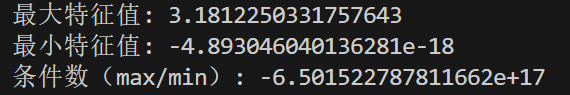
\includegraphics[width=0.6\textwidth]{正则化前条件数.png}
\end{center}

为了解决这个问题,我采用了岭回归的思想,用小量$\epsilon=0.05$对矩阵进行正则化,防止模型被数据中一些"非本质的波动"干扰.

正则化后的条件数和精度分别如下,可以发现加入正则化之后模型分类效果变得很好:

条件数:
\noindent
\begin{center}
    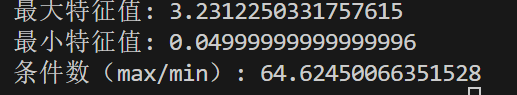
\includegraphics[width=0.6\textwidth]{正则化后条件数.png}
\end{center}
精度:
\noindent
\begin{center}
    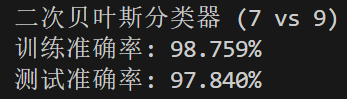
\includegraphics[width=0.6\textwidth]{正则化后精度.png}
\end{center}


\end{document}
